\chapter{Open Air Museum} % senza numerazione
\label{Open Air Museum}

\vspace{5mm}

\section{App native}\vspace{5mm}

L’applicazione consiste in una guida turistica e multimediale in grado di mostrare ai suoi utenti una serie di punti di interesse collegati da percorsi preimpostati. Ogni punto dispone di un pacchetto multimediale di audio e immagini oltre ad una descrizione, un nome e delle informazioni tutte gestibili e configurabili in varie lingue. Tali punti possono essere navigati attraverso applicativi esterni di navigazione per smartphone - sfruttando la geolocalizzazione del dispositivo - oppure attraverso la modalità Esplora dell’applicazione. Quest'ultima permette, una volta attivata, di essere notificati automaticamente sulla presenza di punti di interesse nella zona circostante, dando la possibilità o meno, all’utente, di richiedere informazioni aggiuntive. \vspace{5mm}

Questo è possibile grazie a due componenti: la tecnologia iBeacon\cite{iBeacon}, che verrà descritta nel dettaglio successivamente, e il \emph{background processing}. Quest'ultimo è stato implementato mediante la registrazione di una \emph{background task} per la localizzazione. Tale procedura permette all'applicativo di registrare all'interno del sistema operativo una finestra di esecuzione dedita a quell'operazione specifica. Questo genere di implementazione permette di risparmiare batteria, essendo controllabile quasi interamente dal sistema operativo, che nel caso in cui necessitasse di nuove risorse, potrebbe postporre l'esecuzione della task in background.

\section{iBeacon}\vspace{5mm}

La modalità \emph{Esplora} citata nella sezione precedente è stata implementata sfruttando la tecnologia iBeacon basata su Bluetooth 4.0\cite{Bluetooth}. Essa permette al dispositivo di percepire l’ingresso in una specifica area, marcata da un piccolo radiofaro bluetooth, il quale è collegato a uno determinato punto di interesse dell'applicazione.\vspace{5mm}

\subsection{UUID, major e minor}\vspace{5mm}

La metodologia con cui viene identificata una zona rispetto ad un altra si basa sulla firma del Beacon, ovvero attraverso i suoi tre parametri identificativi: UUID, major e minor. Il primo è una stringa alfanumerica a 128 bit che ha lo scopo di identificare un gruppo di Beacon, mentre gli ultimi due permettono di identificare i Beacon singolarmente. Per questo motivo, un gruppo di Beacon possiede il medesimo UUID ma differisce per major e minor. Questo tipo di stratagemma è utilizzato per identificare una Regione (Region) che viene utilizzata come area di ricerca.\vspace{5mm}

\subsection{Region}\vspace{5mm}

Una \emph{Regione} può essere definita mediante i parametri identificativi dei Beacon e permette di eseguire la ricerca o \emph{Ranging} solo sui Beacon che rispettano i parametri utilizzati durante la definizione della stessa. In particolare, creando una regione con uno specifico UUID, la procedura di ricerca rileverà soltanto i dispositivi con la stessa stringa alfanumerica. Questo è vero anche per major e minor. L'utilizzo di questi tre parametri permette quindi di definire molteplici regioni diverse.

\subsection{Ranging e Proximity}\vspace{5mm}

Esistono due diversi sistemi di approccio alla ricerca in una specifica regione. Il \emph{Ranging} fornisce un interfaccia per ottenere una lista ordinata di Beacon che si trovano nelle vicinanze del dispositivo. La lista è ordinata per distanza dallo smartphone: il Beacon più lontano si troverà nell'ultima posizione e quello più vicino nella prima. La ricerca tramite Proximity, invece, non fornisce informazioni sui Beacon specifici nelle vicinanze ma è utilizzata soltanto per identificare o meno l'ingresso in una regione.\vspace{5mm} 

Open Air museum utilizza solamente il primo parametro per identificare la regione di ricerca, quindi tutti i dispositivi Beacon sono impostati per utilizzare quello specifico UUID. Mentre per il protocollo di ricerca utilizza il Ranging perché permette un controllo più preciso sui dispositivi nelle vicinanze.

\section{Software gestionale}\vspace{5mm}

	Attraverso l’applicativo in Filemaker, esposto tramite un’interfaccia web, i dipendenti del Comune potevano gestire l’inserimento dei punti e dei percorsi, compresi di media e testi relativi. \vspace{5mm}
	
La visualizzazione dei punti avviene attraverso due schermate: la prima è una lista che mostra tutti i punti di interesse con la possibilità di entrare nel dettaglio e modificare le informazioni del punto selezionato e i contenuti multimediali associati ad esso; la seconda mostra l'elenco di tutti i percorsi disponibili e il dettaglio di ognuno di essi, contenente l'elenco dei punti da cui è composto e l'ordine di visita relativo. Per ogni testo vi è la possibilità di fornire una traduzione in tutte le lingue supportate dall'applicativo: italiano, tedesco, inglese, spagnolo e cinese semplificato.\vspace{5mm}

Filemaker mette a disposizione un interfaccia drag and drop per la creazione della parte visuale dell'applicativo, permettendo di collegare i vari elementi trascinati nell'area di lavoro ad una specifica entry del database. Tale interfaccia viene quindi tenuta sempre in sincronia dal motore di Filemaker per riflettere i dati contenuti nel database: questo permette di avere un interfaccia facilmente modificabile e una raccolta dati consistente.\vspace{5mm}

Il vantaggio principale dell'utilizzare questo genere di software si è trovato nella possibilità di convertirlo in una web application, con cui siamo stati in grado di fornire al Comune una piattaforma, senza particolari requisiti di utilizzo, per il caricamento dati. Tale scelta si è rivelata vincente vista la grande frammentazione dei dispositivi in uso negli uffici della suddetta P.A.

\section{Server}\vspace{5mm}
	
La parte server, invece, espone delle Rest API che forniscono sia i dati dell'applicazione che un servizio di autenticazione mediante Json Web Token\cite{JWT}. Questo applicativo è stato sviluppato senza l’ausilio di framework esterni sia per il routing e la gestione dell’autenticazione che per la generazione dei token di sessione.\vspace{5mm}

 Vista la grande quantità di file e la tipologia di dati da servire, è stato scelto NodeJs per la sua efficienza nelle operazioni di I/O rispetto ad una tecnologia più canonica come PHP\cite{PHP} o Java\cite{Java}. L'implementazione di Nodejs di un I/O non bloccante\cite{BlockingVsNonBlocking} risulta in un invio più efficiente di file di medie dimensioni come audio o immagini, e un minor utilizzo di risorse. Tali media sono serviti utilizzando il file system come base, e mediante l'interfaccia messa a disposizione da Nodejs, vengono serviti attraverso una specifica API HTTP\cite{http}. I media sono salvati all'interno di un database MySql attraverso il percorso che hanno nel file system rispetto alla radice del progetto.\vspace{5mm}
 
  Questo approccio permette di svincolare il database da una task onerosa come quella di dover convertire i file ricevuti in base64 e di doverli salvare come entry tabellari. Tale procedura inserisce una criticità: i dati presenti nella memoria possono non riflettere quelli salvati a database e vice versa, perchè non vi è una correlazione diretta fra i due. Le API sono state disegnate per simulare questa correlazione, e ciò, coadiuvato da un blocco di operazioni di lettura e scrittura nella specifica directory, mantiene i media e i dati a database in sincronia. \vspace{5mm}

L'autenticazione, come anticipato in precedenza, avviene attraverso una tecnica chiamata Json Web Token\cite{JWT}, che consiste in uno standard open source basato su JSON per la creazione di token di accesso. Questi token sono firmati per essere piccoli e criptati mediante una chiave privata, cosi da essere decodificati solamente dalle parti autorizzate. Sono generati per essere URL-safe e per eseguire piccole transazioni di dati o per approvare un autorizzazione.  \vspace{5mm}

Nel caso di Open Air Museum vengono utilizzati per validare l'autenticazione: fin quando un token resta valido, cioè finchè la sua data di scadenza non è maggiore della data della richiesta, il client che lo conserva può utilizzarlo per autenticare tutte le richieste http. Per fare questo, l'header di ogni richiesta http dovrà contenere la chiave 'Authorization' con valore 'Bearer' seguito da uno spazio e dal token. Tale autenticazione implementa lo standard RFC 6750: OAuth 2.0 Bearer Token\cite{Bearer}.

\begin{figure}[h]
\centering
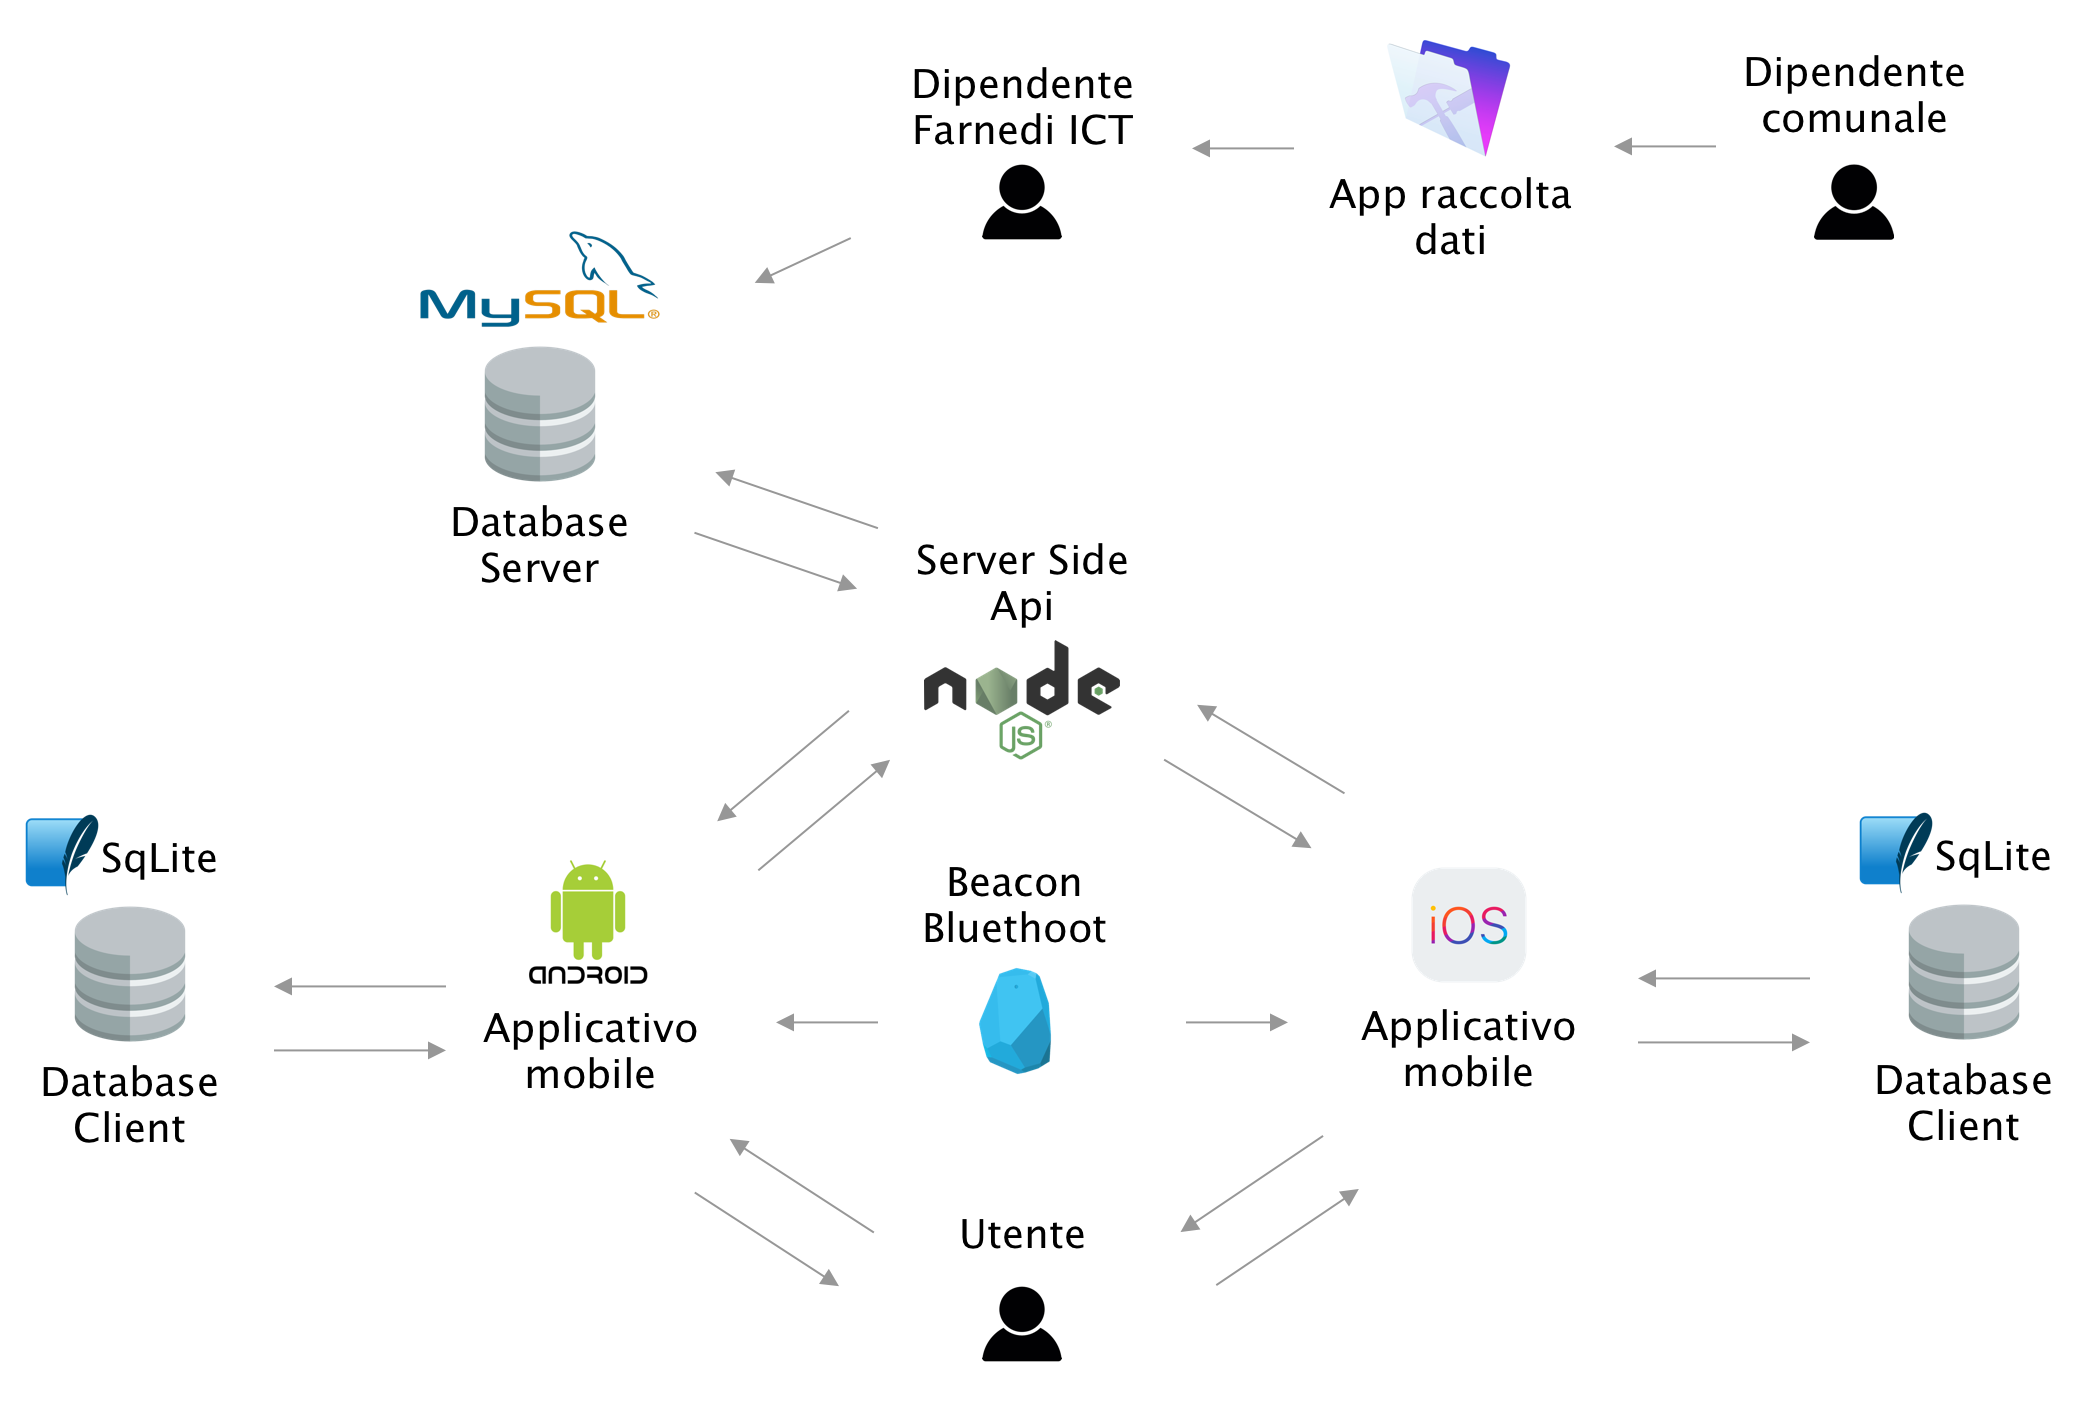
\includegraphics[width=0.8\textwidth]{images/SchemaOpenAirMuseum.png}
\caption{Schema logico dello stack di Open Air Museum}
\end{figure}

\section{Modelli ER}\vspace{5mm}
		
	Il lato server utilizza come database relazionale MySql, che viene sfruttato attraverso un interfaccia Javascript che permette di connettersi al database creando query e inviandole mediante questa connessione. Tutto questo in modo asincrono. Lo schema relazionale per il lato server è presentato in figura 1.2.\vspace{5mm}
	
	Per quanto riguarda le due applicazioni mobile, viene utilizzato sempre un database relazionale, ma sfruttando SqLite come tecnologia, che risulta essere più leggera e adatta a essere eseguita su dispositivi dalle prestazioni ridotte. La figura 1.3 mostra lo schema relazionale per il lato mobile.\vspace{5mm}

Come si può vedere, la gestione delle funzionalità multilingue dei punti e dei percorsi avviene attraverso una relazione da uno a molti con la tabella 'language'. Questa tabella contiene tutti i testi per lingua supportata. Tale accorgimento è assente nello schema relazionale dei dispositivi mobili dato che, al cambiamento della lingua, le nuove traduzioni verranno scaricate dalle Rest API fornite a lato server.


\begin{figure}[h]
\centering
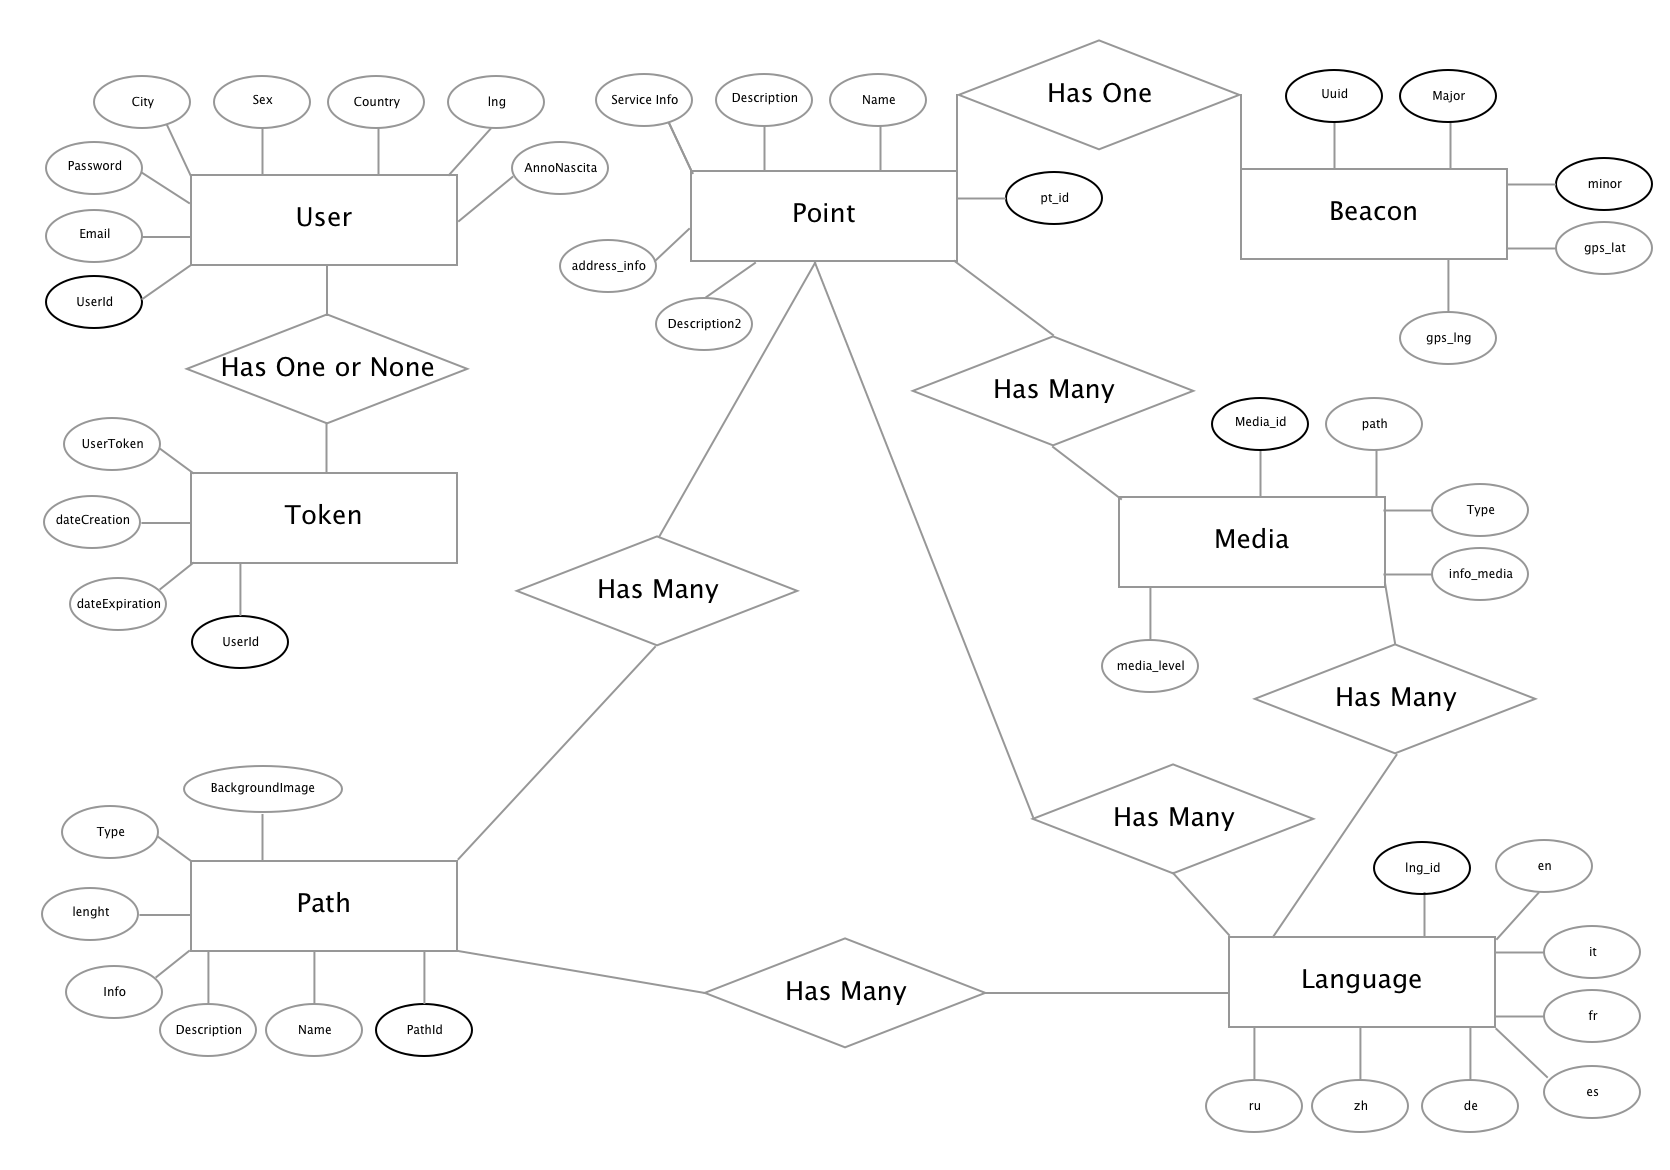
\includegraphics[width=0.8\textwidth]{images/erOld.png}
\caption{Schema ER vecchia versione server}
\end{figure}

\begin{figure}[h]
\centering
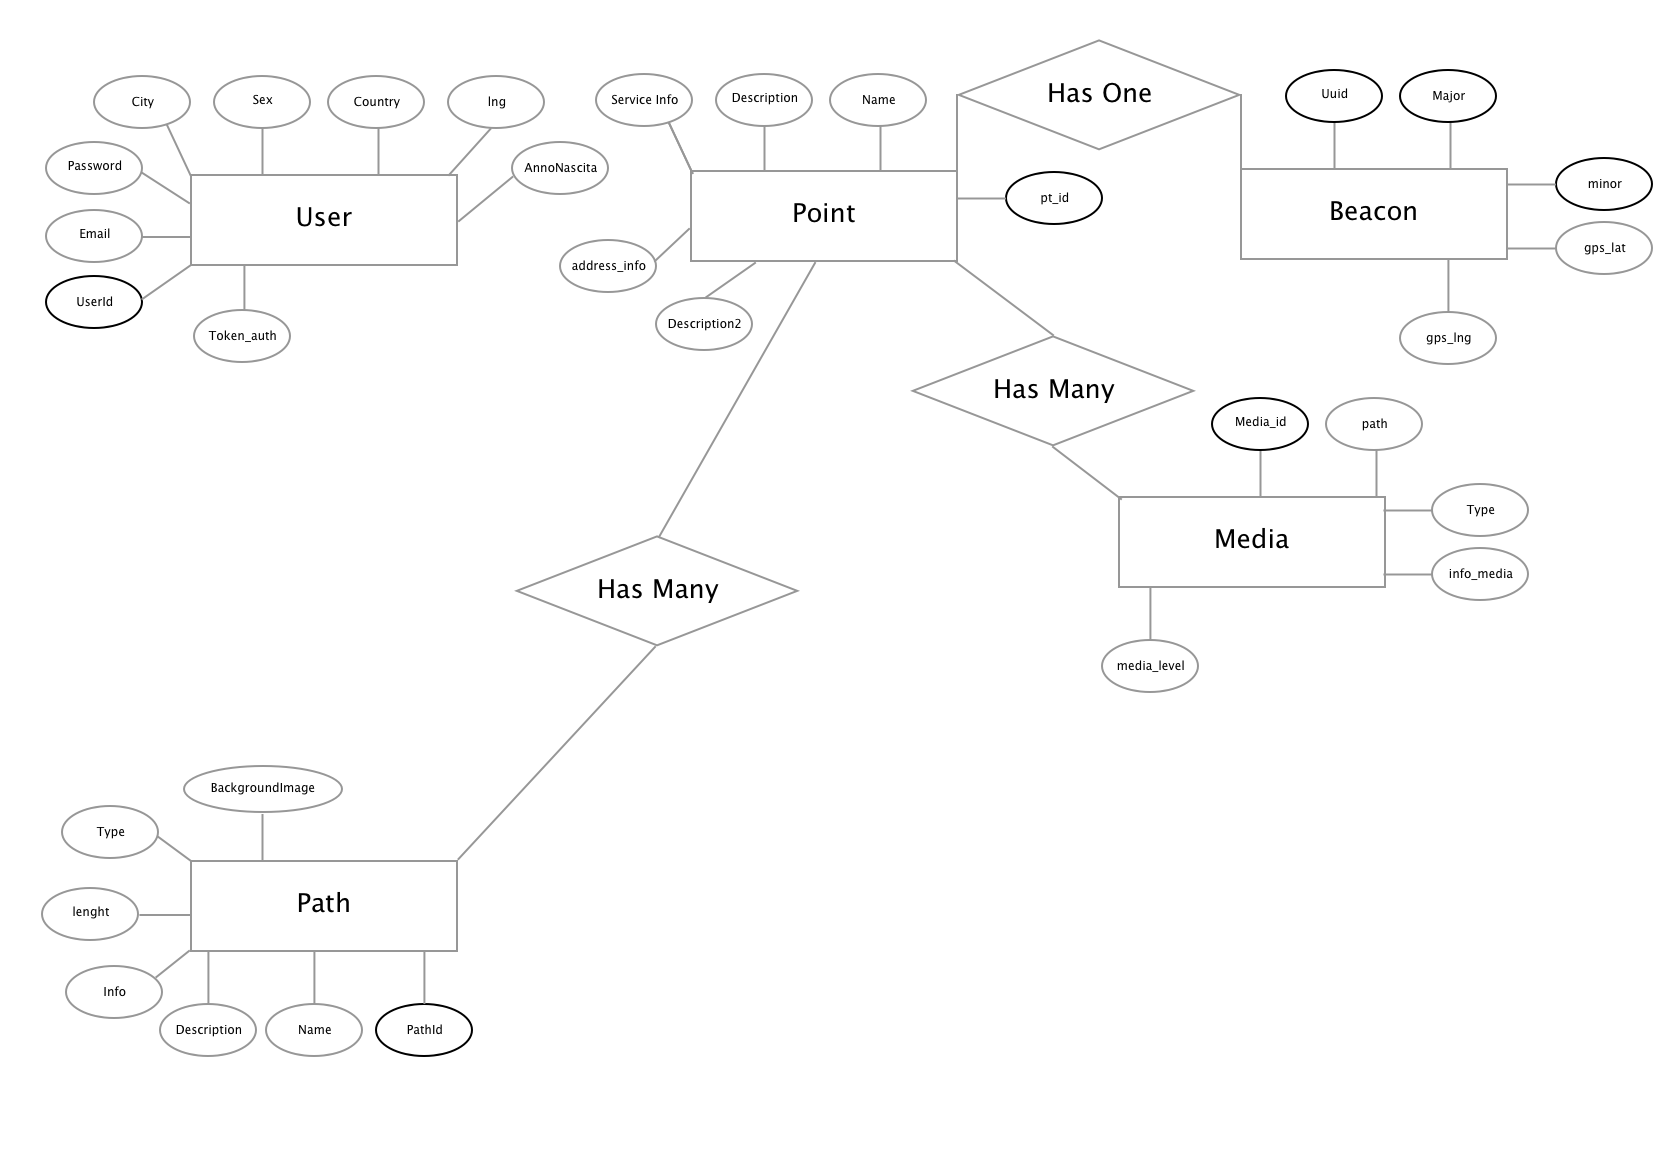
\includegraphics[width=0.8\textwidth]{images/erOldSpartphone.png}
\caption{Schema ER vecchia versione smartphone}
\end{figure}
\vspace{5mm}






